\chapter{Background}

\section{vroom}
vroom is a userspace NVMe driver written in Rust. As of this writing, it offers high performance and the functionality required for general I/O operations, but it is not yet production-ready. Unlike interrupt-driven drivers, vroom uses polling to determine the state of the I/O operations. Polling is often preferable in high-performance applications, as interrupts are relatively performance-intensive operations \cite{spdksubmitting}.
When using vroom without the IOMMU, the device registers are accessed via the pseudo-filesystem \texttt{sysfs}. Direct memory access is performed on hugepages using physical addresses.

An NVMe driver consists of submission and completion queues implemented as ring buffers. The driver adds commands to the submission queue, which the NVMe controller reads and executes. The executed command gets placed on a corresponding completion queue. A deeper explanation of the steps will be provided in \autoref{c:impl}.
As vroom does not have a kernel driver part that can bind to the driver slot, we unbind the kernel driver and bind it to Pci-stub. Pci-stub is a dummy driver that occupies the PCI driver such that the kernel or another application cannot bind to the device.

\section{Memory Management Unit}
Memory Management Units (MMU) for the CPU have been used since the 1980s. After their first integrated application featuring on Intel's 80286 chip \cite{intel80286}, they have since become the de facto standard for addressing computer memory. By providing processes with virtual addresses instead of physical addresses, every process is isolated and only has access to memory assigned to its virtual address space. Each translated address points to a region of memory called a page. These pages can have different sizes, with the default being \qty{4}{\kibi\byte} pages on modern x86-64 architectures.

The translations of these pages are stored in so-called page tables. As one page table does not offer enough address space, multiple tables are linked together, consisting of pointers to a lower-level page table. One page table walk thus includes fetching multiple tables from memory, resulting in a high latency. To avoid performing a page walk every time an address is used, a Translation Lookaside Buffer (TLB) is used to cache translations.

The TLB is very performant to access. Frequent access to the same address can be done at a fraction of the time needed for a page table walk. A TLB miss describes the scenario in which a physical address needs to be translated, but it has no entry in the TLB, resulting in an expensive page walk.

\section{I/O Memory Management Unit}
The advantages and success of the CPU's MMU and the introduction of the PCIe bus specification have incentivized hardware manufacturers to apply this concept to peripheral device buses. In 2006, Intel introduced their "Virtualization Technology for Directed I/O" (Intel VT-d) and AMD their "AMD I/O Virtualization Technology" (AMD-Vi/IOMMU). In this thesis, the term IOMMU references both technologies. The IOMMU was originally only used for "solving the addressing problems of devices with limited address space" \cite{vfiokerneldocs}, but nowadays is used mainly for virtualization and device isolation.

The IOMMU works similarly to the MMU, but instead of mapping memory to a process's virtual address space, it maps it to an I/O virtual address space for device access. The addresses used are called I/O Virtual Addresses (IOVA).

The IOMMU, like the MMU, has a TLB called the I/O Translation Lookaside Buffer (IOTLB). The size of the IOTLB is not officially documented by Intel nor AMD \cite{iommuhuber}.

\begin{figure}[H]
    \centering
    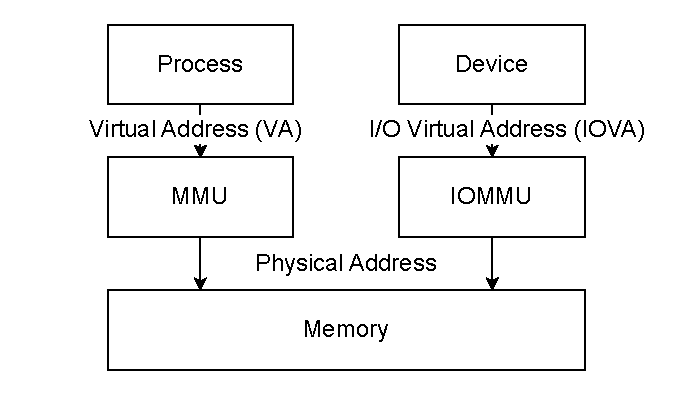
\includegraphics[width=0.6\textwidth]{figures/MMUIOMMU.pdf}
    \caption{MMU and IOMMU relation to physical memory, adapted from \cite{iommuscalability}}
    \label{fig:mmuvsiommu}
\end{figure}

The IOMMU paging structures of Intel's VT-d consist of \qty{4}{\kibi\byte} page tables storing 512 8-byte entries. The IOMMU uses the upper portions to determine the location of the stored page tables and the lower portion of the address as page offset. In the case of \qty{4}{\kibi\byte} pages this offset consists of 12 bits, for \qty{2}{\mebi\byte} pages it consists of 21 bits.
In \autoref{fig:pagewalk}, a 4-level page table structure for translating a 48-bit address to a \qty{4}{\kibi\byte} page with Intel VT-d is shown. A page table walk for one \qty{4}{\kibi\byte} page results in four memory accesses.

\begin{figure}[H]
    \centering
    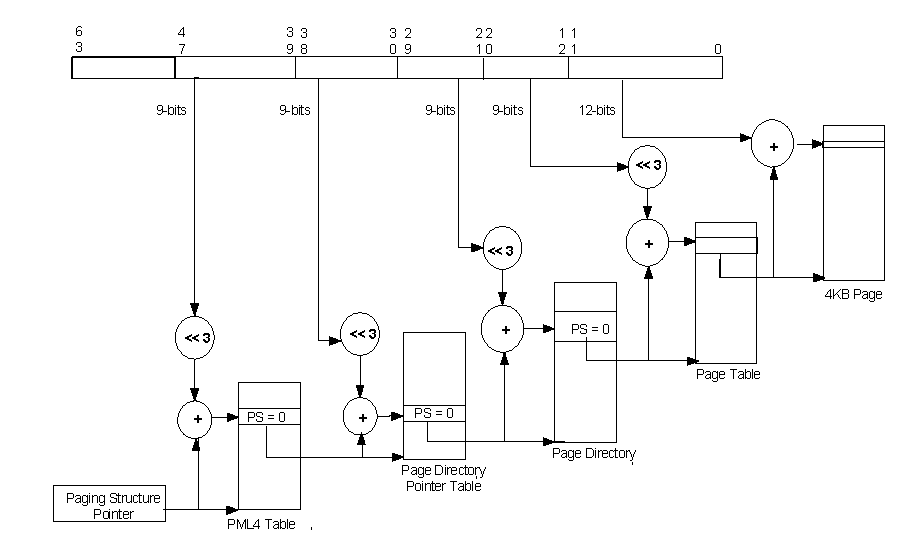
\includegraphics[width=0.9\textwidth]{figures/4kibtranslation.pdf}
    \caption{Intel VT-d Paging structure for translating a 48-bit address to a \qty{4}{\kibi\byte} page, from \cite{vtdspec}}
    \label{fig:pagewalk}
\end{figure}

\section{Direct Memory Access}
Using Direct Memory Access, we can bypass the CPU for I/O operations. Previously, this was handled by a separate DMA-controller hardware (third-party DMA), but using PCI, we can directly access it through bus mastering (first-party DMA) \cite{maellmann}. Using the IOMMU, the request is intercepted and translated to the physical address.

\section{Hugepages}
As the demand for bigger memory mappings, e.g., for big files, increased, the amount of TLB cache misses rose proportionally. With modern CPUs, a TLB typically has space for only 4096 \qty{4}{\kibi\byte} pages, and so, only an address space of \qty{16}{\mebi\byte} can be stored and accessed quickly \cite{emmerich2019user}. To increase the virtual memory space, hardware producers reacted by providing bigger page sizes on their architectures than the default \qty{4}{\kibi\byte}.
Linux currently provides two ways of using Hugepages.
In the optimal case, using a \qty{2}{\mebi\byte} or \qty{1}{\gibi\byte} page size should result in a 512- or 262144-times reduction in cache misses compared to \qty{4}{\kibi\byte} pages. This makes a huge difference, especially in high-performance computing.

\begin{itemize}
    \item \textbf{Persistent Hugepages}: Persistent Hugepages are reserved in the kernel and cannot be swapped or used for another purpose \cite{hugetlbkerneldocs}. These hugepages can be mounted as a (pseudo) filesystem called \texttt{hugetlbfs}. The amount and size of the pages can be specified either during boot on the kernel command line with, e.g., \texttt{hugepagesz=1g hugepages=16} or dynamically using the Linux \texttt{proc} virtual filesystem \cite{hugetlbkerneldocs}.
    \item \textbf{Transparent Hugepages}: Transparent Hugepages (THP) are a more recent addition to the kernel. THPs are not fixed or reserved in the kernel and therefore provide a way of utilizing the TLB effectively without reserving vast amounts of memory \cite{transhugekerneldocs}.
\end{itemize}

vroom currently uses hugepages for DMA and locks them with the Linux syscall \texttt{mlock} to prevent the kernel from swapping them out. When using \qty{4}{\kibi\byte} pages with \texttt{mlock}, it is not guaranteed that the kernel does not migrate the page to another physical location. This is the reason why persistent hugepages have to be used. The kernel cannot move these pages like \qty{4}{\kibi\byte} pages. Other userspace drivers like SPDK or DPDK also rely on this to perform DMA without the IOMMU.

\section{Peripheral Component Interconnect Express}
PCIe is a standard for peripheral device buses. Each device on the PCI bus has a unique PCI address, segmented into three parts, as seen in \autoref{fig:pciaddress}.

\begin{figure}[H]
    \centering
    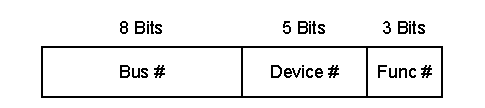
\includegraphics[width=.7\textwidth]{figures/pciaddress.pdf}
    \caption{Segmented PCI identifier}
    \label{fig:pciaddress}
\end{figure}

Each device on the bus uses a PCIe configuration space, which includes registers for controlling the device's behavior, e.g., enabling DMA in the command register. It also includes the Base Address Registers (BAR), which are used to access the device's actual controller. The configuration space can be seen on \autoref{fig:pciconfig}. The marked fields are needed for vroom.

\begin{figure}[H]
    \centering
    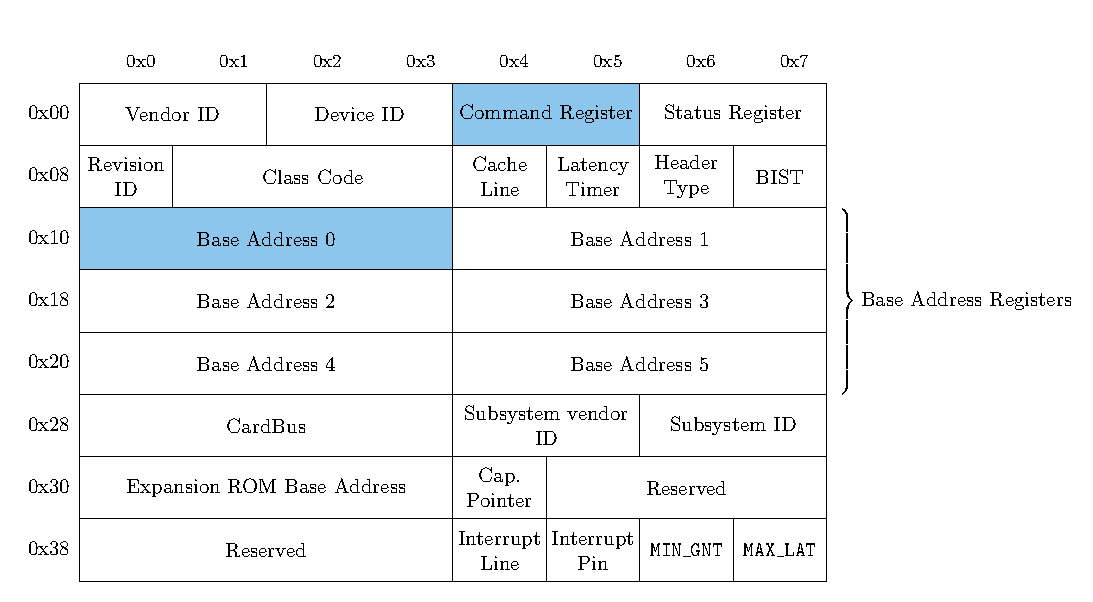
\includegraphics[width=\textwidth]{figures/pcie-config-space}
    \caption{PCIe configuration space, adapted from \cite{vroom}}
    \label{fig:pciconfig}
\end{figure}

\section{Rust}
While userspace drivers can be written in any language having access to syscalls and aligned structs, as proven by the network driver Ixy \cite{ixylanggithub}, Rust excels as it offers high performance and memory safety without garbage collection. This is especially important, as garbage-collected languages have overhead and latency spikes, which can lower performance. Another critical factor is that, like C, Rust does not use exceptions. Being forced to handle errors ensures that no unhandled exception can take down critical code infrastructure.
Additionally, Rust provides low-level access while offering a high-level development experience through zero-cost abstractions.
